\documentclass{article}
\usepackage[final]{neurips_2019}
\usepackage{morris}

% Some update to the NIPS template
\bibpunct{[}{]}{;}{n}{}{,}
\makeatletter
\renewcommand{\@noticestring}{Deep Learning, Sommer 2019, Universiteit van Amsterdam}
\makeatother

\renewcommand{\thesubsubsection}{\alph{subsubsection})}

\title{Assignment 3. Deep Generative Models}
\author{%
  Maurice Frank\\
  11650656\\
  \href{mailto:maurice.frank@posteo.de}{maurice.frank@posteo.de} \\
  Code: \href{https://github.com/morris-frank/uvadlc_practicals_2019/tree/master/assignment_2}{github}
}

\begin{document}
\maketitle

\section{Variational Auto Encoders}
We have:
\begin{description}
  \item[\(\mathcal{D}={\{\B{x}_n\}}^N_{n=1}\)] the dataset
  \item[\(\B{x}_n\in{\{0,1\}}^M\)] one datapoint, from Bernoulli distribution
\end{description}

\subsection{Variational autoencoders vs standard autoencoders}
Let us first note down the two objectives of the VAE and a standard sparse autoencoder~\cite{doersch2016}, respectively:

\begin{align}
  \E_{q(z|\B{x}_n)}[\log{p(\B{x}_n|Z)}] &- D_{KL}(q(Z|\B{x}_n)||p(Z))\\
  {||D_{AE}(E_{AE}(\B{X})) - \B{X}||}^2 &+ \λ||E_{AE}(\B{X})||_0
\end{align}

For the sparse autoencoder we use \(D_{AE}, E_{AE}\) for the Decoder model and Encoder model and \( \λ \) is our regularization hyperparameter.
The main similarity between both is that they have the encoder and decoder pair.
The encoder encodes the data into a smaller latent space and the decode generates samples from this space back into our datasets space \(X\).

\subsubsection{How do they differ in their main function?}
We see that both methods vary considerably in their main optimization objective.
The VAE objective includes modeling the intractable encoding distribution\(p(Z|X)\) through the surrogate \(q(Z|X)\).
The standard autoencoder on the other side does not actually model the encoding distribution but only has the reconstruction capabilities of those encodings as its objective.

\subsubsection{Is the standard autoencoder a generative model?}
The standard autoencoder is not a generative model as one cannot sample from the implicit latent space.
We do have the latent representation and thus can vary the input into the decoder but this does not relate to sampling from the latent manifold of all possible encodings.
We can sample from the space the encodings live in but as we do not model the actual distribution this is not a generative model.

\subsubsection{Can the VAE be a drop-in replacement for a normal autoencoder?}
The VAE can be a drop-in replacement for the standard autoencoder in respective applications.
Autoencoders are used for compression as they can reduce the input data into the smaller informative latent space.
The VAE does do they same and can be used for the same.
Further autoencoders can denoise data by mapping the noisy data close to the noise-less data in the latent space.
Again the VAE can do the same.
Generally the addition of the VAE is enforcing the continuity of the latent space by introducing \(q(\·)\).
While this opens up new (see generative) applications it does not restrictive the former.

\subsubsection{Why does VAE generalize better?}
The standard autoencoder is missing the is not modelling the encoding distribution.
In the VAE our \(q(Z|X)\) forces the latent space to be continuos.
As such interpolating in the latent space does correspond to interpolating in the data space.
During training we therefore build a latent space that is better capable to handling unseen data and can therefore also generalize beyond the trainings data.

\subsection{How to sample from \(p(Z)\)?}
We sample using ancestral sampling.
First we sample \(\B{z}_i\sim p(\B{z}_n) = \N(0,\1_D)\).
We put this sample into the Decoder \(f_\θ(\·)\) to get our parameters for the bernoulli distribution.
Than we sample each pixel from each bernoulli \(\text{pixel}_m \sim \text{Bern}(\B{x}_n^{(m)}|{f_\θ(\B{z}_n)}_m)\) to get the sample from the joint distribution.

\subsection{Why is the assumption of \(p(Z)\) not restrictive?}
Our assumption that \(p(Z)\) is a standard-normal distribution does not hinder us from learning a complex manifold for \(X\) as we transform it using \(f_\θ(\·)\).
Thus the complexity lies in the mapping from latent \(z\)-space and \(x\)-space.

\subsection{Evaluating \(\log p(\B{x}_n)\)}
\subsubsection{Approximating using Monte-Carlo}
We can sample from our distribution of \(\B{z}_n\) to compute the integral for one \(\B{x}_n\):
\begin{align}
  \log{p(\B{x}_n)}
  &= \log \int p(\B{x}_n|\B{z}_n)p(\B{z}_n)\,d\B{z}_n\\
  &\approx \log \÷{1}{n} \Σ_{i=1}^{n} p(\B{x}_n|\B{z}_i),\quad \B{z}_i\sim p(z)
\end{align}

\subsubsection{Why is Monte-Carlo integration here inefficient?}
We sample from \(p(Z)\).
As we nee the integral for each datapoint this is inefficient with any non trivial dimensionality in \(Z\).
The precision of our density estimation of \(p(\B{x}_n|\B{z}_n)\) decreases exponentially as the dimension of \(\B{x}_n\) increases.
As such we would need to increase the number of samples exponentially with higher dimension of \(\B{z}_n\) to keep the estimation precise.
In the real world the hidden embeddings often has hundreds of dimensions.
A density dimension that we would have to do for every single input in every inference step is too inefficient to be usable.

\subsection{Kullback-Leibler divergence of Gaussians}
We assume: \(q = \N(\μ_q, \σ_q^2),\quad p=\N(0,1)\)

\subsubsection{Two examples of KL-divergence}
Checking with the closed form solution in Section~\ref{sec:kl_closed_form} we see as expected that the divergence is zero for \( \σ_q = 1, \μ_q = 0\) and increases for any deviation from either of those values:
\begin{align}
  \t{Big:}&\quad(1 + 10^{5}, 10^{5}) \⇒ D_{\t{KL}}(q||p) = \num{1.0d10}\\
  \t{Small:}&\quad(1 + 10^{-5}, 10^{-5}) \⇒ D_{\t{KL}}(q||p) = \num{1.49d-10}
\end{align}

\subsubsection{Closed-form solution of the KL-divergence}%
\label{sec:kl_closed_form}
\begin{align}
  q(x) &= \÷{1}{\sqrt{2\π}\σ_q} \exp{\left[-\÷{1}{2}{(\÷{x-\μ_q}{\σ_q})}^2\right]}\\
  p(x) &= \÷{1}{\sqrt{2\π}} \exp{\left[-\÷{1}{2}x^2\right]}\\
  D_{\t{KL}}(q||p)
  &= -\E_{q(x)}\left[ \log{\f{p(x)}{q(x)}} \right]\\
  &= -\E_{q(x)}\left[ \log{(\÷{1}{\sqrt{2\π}})} -\÷{1}{2}x^2 -\log{(\÷{1}{\sqrt{2\π}})} +\log{\σ_q} +\÷{1}{2}{(\÷{x-\μ_q}{\σ_q})}^2 \right]\\
  &= -\E_{q(x)}\left[ \÷{1}{2}({\left(\÷{x-\μ_q}{\σ_q}\right)}^2 - x^2)\right] - \E_{q(x)}\left[\log{\σ_q}\right]\\
  &= -\÷{1}{2}\E_{q(x)}\left[{\left(\÷{x-\μ_q}{\σ_q}\right)}^2 - x^2\right] - \log{\σ_q}\\
  &= -\÷{1}{2}\left(\÷{1}{\σ_q^2}\E_{q(x)}[{(x-\μ_q)}^2] - \E_{q(x)}[x^2]\right) - \log{\σ_q}\\
  &= -\÷{1}{2}\left(\÷{\σ_q^2}{\σ_q^2} -\σ_q^2 -\μ_q^2\right) - \log{\σ_q}\\
  &= \÷{\σ_q^2 + \μ_q^2 - 1}{2} - \log{\σ_q}
\end{align}

\subsection{Why is ELBO a lower bound?}
The evidence lower bound (ELBO) for our VAE is given by:
\begin{equation}
  \E_{q(z|\B{x}_n)}[\log{p(\B{x}_n|Z)}] - D_{\t{KL}}(q(Z|\B{x}_n)||p(Z))
\end{equation}
We want to maximize our data model \(p(\B{x}_n)\), or written including the ELBO:\@
\begin{equation}
  p(\B{x}_n) =  \E_{q(z|\B{x}_n)}[\log{p(\B{x}_n|Z)}
                - D_{\t{KL}}(q(Z|\B{x}_n)||p(Z))]
                + D_{\t{KL}}(q(Z|\B{x}_n)||p(Z|\B{x}_n))
\end{equation}
As KL divergence is strictly \(>0\) we directly see that the ELBO is a lower bound for our actual objective.
Now the distance from the lower bound to the actual evidence is the divergence of our surrogate approximate posterior \(q(Z|\B{x}_n)\) from the actual posterior \(p(Z|\B{x}_n)\).
The lower bound always stays a lower bound so maximizing the lower bound does also maximize the actual objective.

\subsection{Why do we optimize the lower bound instead of the log-probability?}
We must optimize the lower bound as we cannot compute \(D_{\t{KL}}(q(Z|\B{x}_n)||p(Z|\B{x}_n))\).
Computing this divergence would mean we need to compute \(p(z|\B{x}_N)\).
If we could do this we would not have introduced \(q(z|\B{x}_n)\).

\subsection{What can happen if we push ELBO up?}
Basically the two things that can happen is either our data log probability \(\log p(\B{x}_N)\) rises or the divergence between \(q(Z|\B{x}_n)\) and \(p(Z|\B{x}_n)\) gets lower.
Both ways are good for us.
In the first case the likelihood of the trainings data rises meaning we get a better ML model.
The reconstruction gets better.
In the second case our surrogate gets more similar to the actual encoding which means we improve our embeddings.

%Interestingly this fact does imply our model might behave quite differently to what we would expect.

\subsection{How can we name the parts of the loss of an VAE?}
We can write the loss of the VAE as the per-sample sum of the \textit{reconstruction} and the \textit{regularizer} loss:
\begin{align}
  \L^{\t{recon}}_n &= - \E_{q_\φ(z|\B{x}_n)}[\log p_\θ(\B{x}_n|Z)]\\
  \L^{\t{reg}}_n &= D_{\t{KL}}(q_\φ(Z|\B{x}_n)||p_\θ(Z))\\
  \L &= \÷{1}{N}\Σ_{n=1}^N (\L^{\t{recon}}_n + \L^{\t{reg}}_n)
\end{align}

As written before \(\L^{\t{recon}}_n\) gives us the negative data likelihood of the input sample \(\B{x}_n\) using its embedding from the encoder \(q_\φ(\·)\).
In other words this gives us the reconstruction probability of \(\B{x}_n\) using the decoder \(p_\θ(\·)\) under an already set embedding for \(\B{x}_n\), but negative (to get a loss).

Our second objective wants to minimize the divergence of \(q_\φ(Z|\B{x}_n)\) with respect to \(p_\θ(Z)\).
Now that means that every posterior of the encoders input wants to be similar to the distribution of our latent embeddings \(Z\).
Of course this is impossible as in the case of no divergence all posteriors would be the same.
If the model wants to have reconstruction capabilities while minimizing the divergence of the embedding posteriors it is best to map similar inputs to similar posteriors as that allows them to be larger, hence less diverged from the \(p(Z)\).
Further this will lead to a distribution of posteriors as such that:
\begin{equation}
  D_{\t{KL}}\left(\Σ_n q_\φ(Z|\B{x}_n)||p_\θ(Z)\right) \approx 0
\end{equation}
This is exactly what we want as we thus make a partition of the embedding manifold based on latent feature similarity (in the case of MNIST, same number are close).


\subsection{Writing down the complete loss}
We assume for our encoder:
\begin{align}
  q_\φ(\B{z}_n|\B{x}_n)
  &= \N(\B{z}_n|\μ_\φ(\B{x}_n), \diag(\Sigma_\φ(\B{x}_n)))\\
  &= {(2\π)}^{-\÷{k}{2}} {(\Π_i{\Sigma_\φ(\B{x}_n)}_i)}^{-\÷{1}{2}} \exp{(-\÷{1}{2} {(\B{z}_n-\μ_\φ(\B{x}_n))}^T {(\diag\Sigma_\φ(\B{x}_n))}^{-1} (\B{z}_n -\μ_\φ(\B{x}_n)) )}
\end{align}

As we now have a multivariate distribution our derivation of the KL divergence from the standard normal changes slightly:

\begin{align}
  D_{\t{KL}}(q_\φ(Z|\B{x}_n)||p_\θ(Z)) &= \÷{1}{2} \left[ \Σ_i{\Sigma_\φ(\B{x}_n)}_i^{-1} + \μ_\φ^T\μ_\φ - d_z - \log(\Π_i{\Sigma_\φ\B{x}_n)}_i \right]
\end{align}

\begin{align}
  \L^{\t{recon}}_n
  &= -\E_{q_\φ(z|\B{x}_n)}[\log p_\θ(\B{x}_n|Z)]\\
  &\approx -\log p_\θ(\B{x}_n|\B{z}_n)\quad \t{with } \B{z}_n\sim q_\φ (Z|\B{x}_n)\\
  \L^{\t{reg}}_n
  &= D_{\t{KL}}(q_\φ(Z|\B{x}_n)||p_\θ(Z))\\
  &= \÷{1}{2} \left[ \Σ_i{\Sigma_\φ(\B{x}_n)}_i^{-1} + \μ_\φ^T\μ_\φ - d_z - \log(\Π_i{\Sigma_\φ\B{x}_n)}_i \right]\\
  \L
  &= \÷{1}{N}\Σ_{n=1}^N (\L^{\t{recon}}_n + \L^{\t{reg}}_n)
\end{align}

\subsection{The reparametrization trick}
\subsubsection{Why do we need \( \∇_\φ\L \)?}
We need the gradient of our loss with respect to the parameters \( \φ\) of our encoder \(q_\φ(\·)\) for backpropagation.
To update the weights \( \φ\) we need to know their influence on the loss.

\subsubsection{Why can we not compute \( \∇_\φ\L \)?}
We cannot compute this gradient because we sample from \(q_\φ(\B{z}_n|\B{x}_n)\).
As we sample from we cannot attribute the effect of this inference step to and of the weights \( \φ\) in \( \μ_\φ(\·)\) or \(\Sigma_\φ(\·)\).

\subsubsection{How does the reparametrization trick solve that problem?}
The reparametrization trick solves this problem by taking the stochastic non-deterministic sampling operation out of the encoder.
This uses the special property of normal distribution, that:
\begin{align}
  \N(\B{z}_n|\μ_\φ(\B{x}_n), \diag(\Sigma_\φ(\B{x}_n)))
  &= \diag(\Sigma_\φ(\B{x}_n)) \· \N(0, \1_D) + \μ_\φ(\B{x}_n)
\end{align}
The only remaining stochastic process \(\N(0, \1_D)\) is therefore than outside the parameterized model and we can compute the gradient.

\subsection{Building a VAE}
See the code in \texttt{code/vae.py}

\subsection{ELBO during training}
See Figure~\ref{fig:elbo} for the plots of the ELBO curves.

\begin{figure}[]
  \centering
  \begin{tabularx}{\linewidth}{XX}
    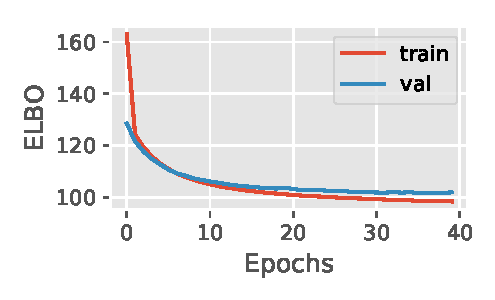
\includegraphics[width=\linewidth]{assignment_3/code/figures/vae_20.pdf} &
    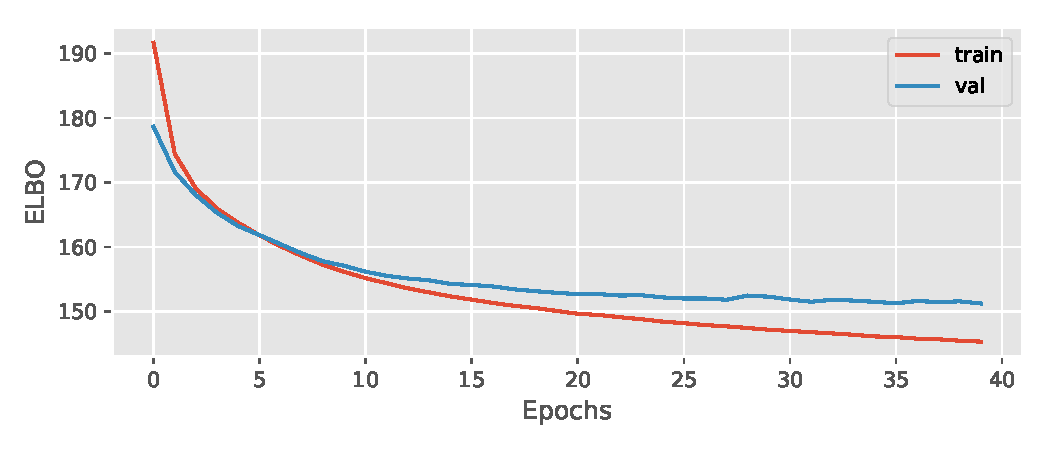
\includegraphics[width=\linewidth]{assignment_3/code/figures/vae_2.pdf}
  \end{tabularx}
  \caption{The ELBO curves of the trainings and validation set for encoding sizes \(z\) of \textit{left} 20 and \textit{tight} 2.}
  \label{fig:elbo}
\end{figure}

\subsection{Samples during training}
See Figure~\ref{fig:vae_samples} for samples of the VAE during training.

\begin{figure}
  \centering
  \begin{tabularx}{\linewidth}{XX}
    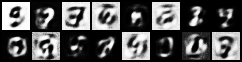
\includegraphics[width=\linewidth]{assignment_3/code/figures/vae_sample_0.png} &
    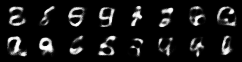
\includegraphics[width=\linewidth]{assignment_3/code/figures/vae_sample_10.png} \\
    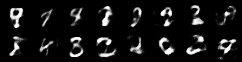
\includegraphics[width=\linewidth]{assignment_3/code/figures/vae_sample_20.png} &
    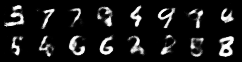
\includegraphics[width=\linewidth]{assignment_3/code/figures/vae_sample_30.png} \\
    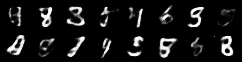
\includegraphics[width=\linewidth]{assignment_3/code/figures/vae_sample_39.png}
  \end{tabularx}
  \caption{Samples drawn from the VAE with encoding size \(20\) at epoch \(0,10,20,30,40\) (from \I{top left} to \I{bottom right}). At each epoch we sample 16 samples from \(p(Z)\).}
  \label{fig:vae_samples}
\end{figure}

\subsection{Manifold during training}
See Figure~\ref{fig:vae_manifold} for three manifolds during training.

\begin{figure}
  \centering
  \begin{tabularx}{\linewidth}{XXX}
    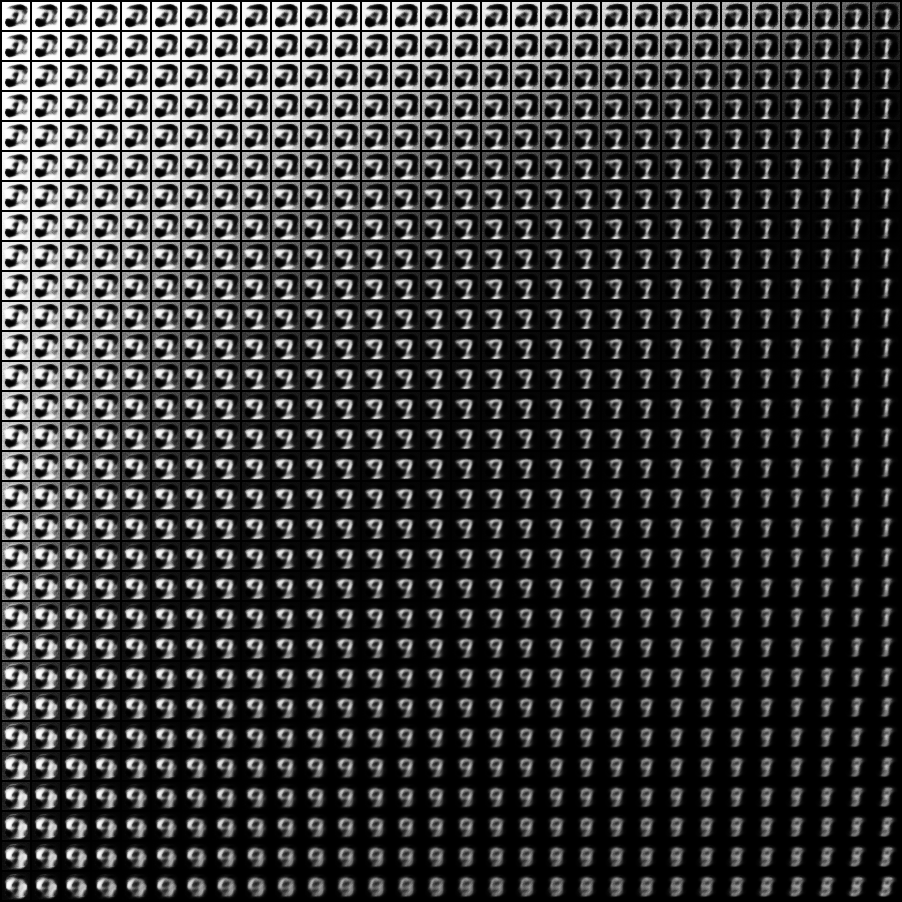
\includegraphics[width=\linewidth]{assignment_3/code/figures/vae_manifold_0.png} &
    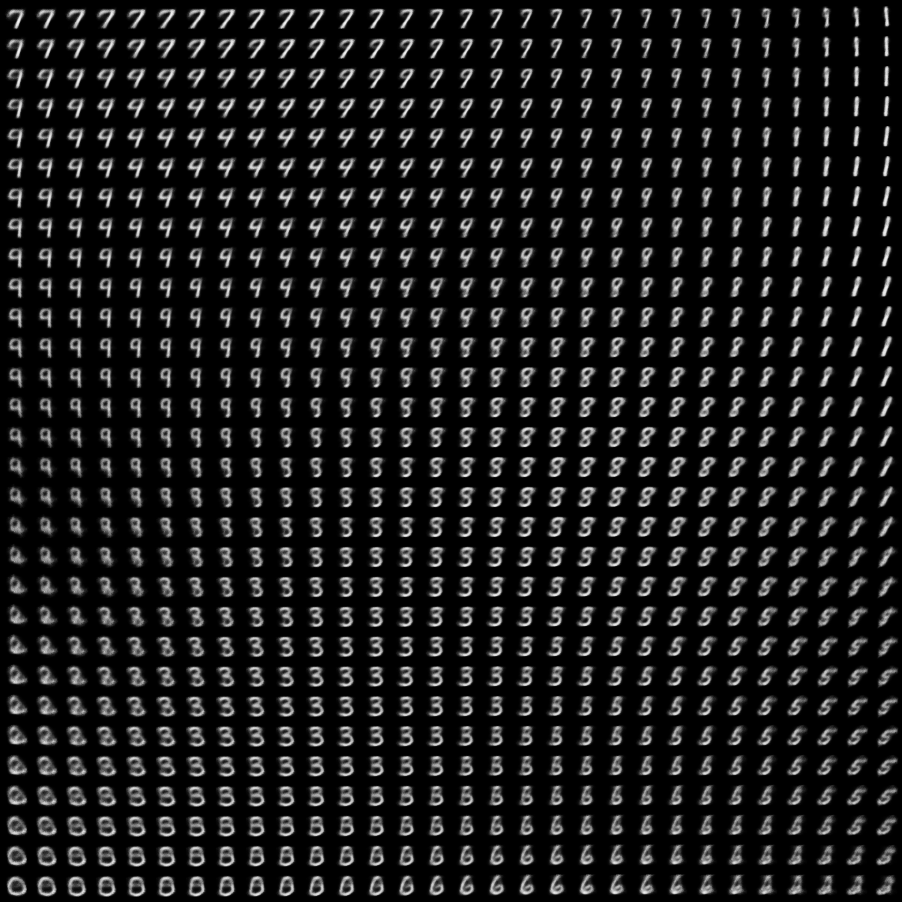
\includegraphics[width=\linewidth]{assignment_3/code/figures/vae_manifold_20.png} &
    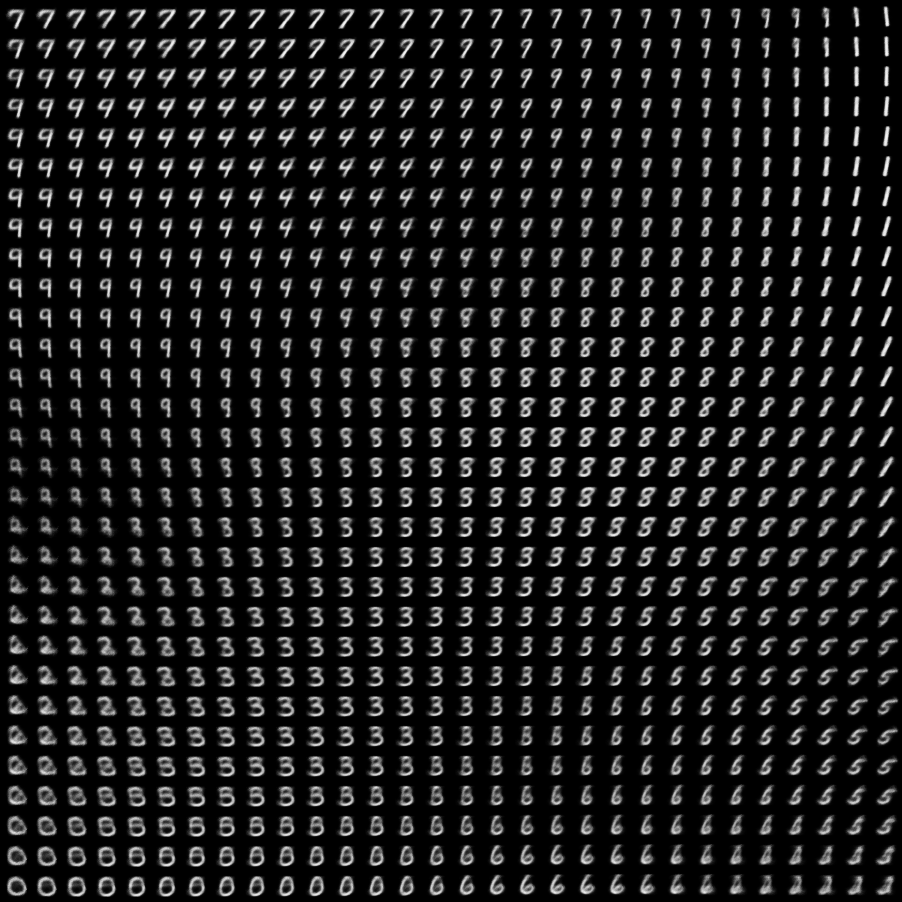
\includegraphics[width=\linewidth]{assignment_3/code/figures/vae_manifold_39.png}
  \end{tabularx}

  \caption{The manifold of the VAE with encoding size \(2\) at epoch \(0, 20, 40\).}
  \label{fig:vae_manifold}
\end{figure}


\section{Generative Adversarial Networks}
We have:
\begin{description}
  \item[\(D(\·)\)] our discriminator function/network
  \item[\(G(\·)\)] our generator function/network
  \item[\(p(\B{z})\)] the noise distribution, here \(\sim \N(0,\1_d)\)
  \item[\(\mathcal{D} = \…, i_i,\… \)] dataset of images, each \(i_i \∈ \ℝ^{h\×w}\)
\end{description}
and our GAN objective:
\begin{equation}
  \min_G \max_D V(D, G) = \min_G \max_D \E_{p_{\t{data}}(\B{x})}[\log D(X)] + \E_{p_z(\B{z})}[\log(1 - D(G(Z)))]
\end{equation}

\subsection{Inputs and outputs of \(D(\·)\) and \(G(\·)\)}
For the Generator we have a randomly sampled input of size \(d\) and an output in image size.
\begin{align}
  \t{input}_G &\sim p(\B{z}) = \N(0,\1_d) \∈ \ℝ^{D}\\
  \t{output}_G &\∈ \ℝ^{h\·w}
\end{align}

For the Discriminator we have an image sized input and a single output.
\begin{align}
  \t{input}_D &\∈ \ℝ^{h\·w}\\
  \t{output}_D &\∈ \ℝ
\end{align}

\subsection{What are the parts of the GANs objective?}
The left part \(\E_{p_{\t{data}}(\B{x})}[\log D(X)]\) is the data likelihood of the trainings data under the discriminator.
Basically it maximizes the discriminators output for samples in the ground truth data set.

The right part \(\E_{p_z(\B{z})}[\log(1 - D(G(Z)))]\) gives the inverse score of the discriminator for sampled \(\B{z}\) that were put through the generator.
The generator wants to minimize this as than outputs are similar for \(p_{\t{data}}\) and \(p_z\).
The discriminator wants to maximize to have reciprocal outputs for the two distributions.

\subsection{How does a converged objective look like?}
If training is converged than the generator produces perfect samples which mean that the distribution of generated samples is equal to the trainings set:
\begin{equation}
  p_{\t{data}}(\B{x}) = G(\B{z})\quad \B{z}\sim p_z(\B{z})
\end{equation}

at that point a perfectly discriminator is no different from randomness as it is impossible to distinguish the two datasets:
\begin{align}
  \E_{p_{\t{data}}(\B{x})}[D(\B{x})] &= \E_{p_z(\B{z})}[D(G(\B{z}))] = \÷{1}{2}\\
  &\⇒\\
  V(D,G) &= \log \÷{1}{2} + \log \÷{1}{2}\\
  &= -\log{4}
\end{align}

\subsection{Why can \(\log(1 - D(G(Z)))\) be problematic?}
In the beginning \(G(\·)\) and \(D(\·)\) are shit.
But than in early training it is easier for the discriminator to differ between real and fake than it is for the generator to fool it.
Hence in our left side objective we get near 0 early on.
This saturating effect makes backpropagation for the generator difficult with the losses near zero.
The solution to this problem is fairly simple.
We separate the two objectives into:
\begin{align}
  \L_D &= -\E_{p_{\t{data}}(\B{x})}[\log D(X)] -\E_{p_z(\B{z})}[\log(1 - D(G(Z)))] \\
  \L_G &=  -\E_{p_z(\B{z})}[\log(D(G(Z)))]
\end{align}
With the changed objective for the generator we averted this problem and as we will update the two models consecutively its is not a problem that we formulated separate objectives.

\subsection{Building the GAN}
See code in \texttt{code/gan.py} for the implementation.

We build the Generator \(G\) as follows:
a linear layer from latent space into a hidden size \(h=128\) followed by three linear layers with adjacent leaky ReLU (with \(\α=0.2\)) and batch normalization, respectively.
Each linear layer doubles the hidden size.
The final linear layer projects down to the inputs image size and we squash the outputs with a tanh.

We build the discriminator \(D\) as two linear layers again each followed by a leaky ReLU (\( \α = 0.2\)) and a dropout layer (\(p=0.3\)) for better regularization.
The first takes the input size down to \(h\·4\) and subsequently to the half.
Finally we have linear classifier with one output and squash this with a sigmoid.

We use optimizer Adam for both models and a fixed learning rate of \(\eta = 5e-4\).
We separate the objectives for better stability as explained before and we sample from \(G\) for each objective again.

\subsection{Sampling from GAN}
Refer to Figure~\ref{fig:gan_samples} for samples taking during the training of our GAN.

\begin{figure}
  \centering
  \begin{tabularx}{\linewidth}{XXXX}
    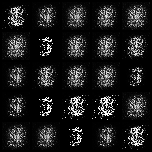
\includegraphics[width=\linewidth]{assignment_3/code/figures/gan_2000.png} &
    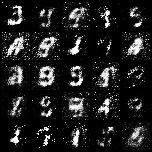
\includegraphics[width=\linewidth]{assignment_3/code/figures/gan_8000.png} &
    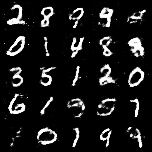
\includegraphics[width=\linewidth]{assignment_3/code/figures/gan_94000.png} &
    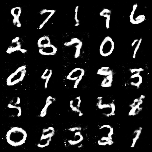
\includegraphics[width=\linewidth]{assignment_3/code/figures/gan_185000.png}
  \end{tabularx}

  \caption{Samples from our GAN implementation during training. From \I{left} to \I{right}: 2 epochs, 8 epochs, 100 epochs, 200 epochs.}
  \label{fig:gan_samples}
\end{figure}

\begin{figure}
  \centering
  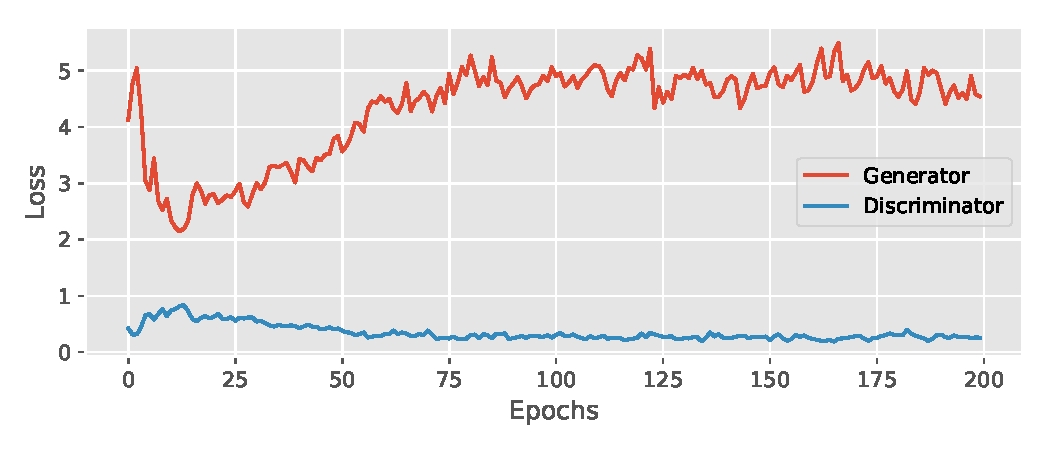
\includegraphics[width=0.6\linewidth]{assignment_3/code/figures/gan.pdf}
  \caption{The loss of the two models \(D\) and \(G\) of the GAN during training.}
  \label{fig:gan_loss}
\end{figure}

\subsection{Interpolation using the GAN}
For an example of interpolating in the latent space of our GAN check Figure~\ref{fig:gan_interpolation}.
We proceed equally to the manifold sampling in the VAE.
We sample uniformly from the unit cube with latent dimensionality of the Generator.
For each marginal dimension we build the equidistant steps (in Euclidean space) and transform the resulting intermediate points with the inverse cumulative density of the normal distribution.

\begin{figure}
  \centering
  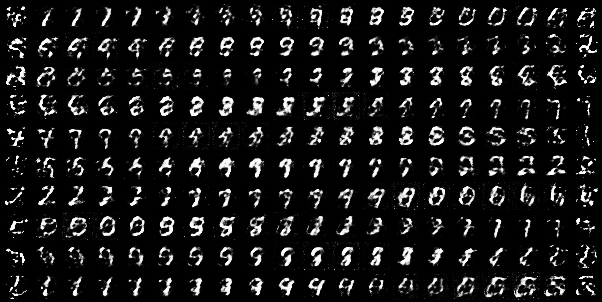
\includegraphics[width=0.9\linewidth]{assignment_3/code/figures/gan_interpolate.png}
  \caption{Equidistant interpolations between different randomly selected points in the latent space. Each row is one interpolation. At each row we sample a new random point and interpolate from the last sample.}
  \label{fig:gan_interpolation}
\end{figure}

\section{Generative Normalizing Flows}
\subsection{Update equation for the \textit{multivariate} flow}
In our flow model we are using an invertible function \(f(\·): \ℝ^m \rightarrow \ℝ^m\) to map an input \(\B{x}\) to its next step \(\B{z} = f(\B{x})\) (therefore \(x = f^{-1}(\B{z})\)).
The transformation \(f(\·)\) changes our density manifold \(p(X)\) of the input.
Now this change can be seen locally as contractions and stretching of the manifold (like pulling around the manifold, intuitively).
The local change of our transformation is exactly its Jacobian \(\pf{f}{\B{x}^T}\).
The change in local volume (the contractions) is the determinant of a transformation and therefore globally the determinant of the Jacobian \(\det \pf{f}{\B{x}^T}\).
Using this we can write the updated density as:
\begin{equation}
  p(\B{x}) = p(\B{z}) \· | \det \pf{f}{\B{x}} |
\end{equation}

For the application of normalizing flows we will chain multiple such mapping to get the final \(p(\B{z})\).
We describe the intermediate states with the hidden states \(\B{h}_i\).
One transformation is then \(\det \pf{\B{h_i}}{\B{h}_{i-1}^T}\).
And thus we can write the complete transformation as:

\begin{equation}
  \log p(\B{x}) = \log p(\B{z}) + \Σ_{l=1}^L \log | \det \pf{\B{h}_l}{\B{h}_{l-1}^T} |
\end{equation}

We use the logarithm for numerical stability as we than have a sum instead of a product.

\subsection{How are the formulas for the multivariate case constrained?}
As given above the function \(f(\·)\) has to map to same dimensionality as the inputs.
Otherwise  the determinant would be zero and we could not find the inverse.
The second constraint is that we have to be actually able to compute the determinant of the Jacobian.

\subsection{What computational problem might arise with this formulation?}
The computational problem with the na\"{\i}ve approach is that we need to compute the determinant of the Jacobian.
Computing the determinant of the Jacobian is at least \(\O(d^3)\)~\cite{rezende2015} (where \(d\) is the size of the hidden units \(\B{h}\)) and we have to do this \(L\) times (for each layer).

\subsection{What changes if the inputs are discrete not continuos?}
Image pixels have discrete values (mostly from the 8-bit intensity set).
Thus our original image distribution \(p(X)\) is equal to the sum of Dirac delta functions.
If we now apply our density contraction transformation on this we will still end up with a set of dirac deltas.
This means our embedding space \(p(Z)\) is also discrete just like a standard autoencoder.
We do want a  continuous regularized embedding space where we can interpolate.

One solution to this problem from~\cite{ho2019} is to add some noise to out discrete input labels.
In our case we would add some noise \(\sim \N(0,1)\) on our image pixels.
The variance acts as a regularization hyperparameter.

\subsection{What is the input and output of the flow model?}
The input to the flow based model is always of the same size (let different batch sizes).
For training we put in the images plus the element wise gaussian noise.
For inference we will got through the computational graph in reverse but because we have the bijective mappings our inputs are still of the image's size.
Now of course for sampling we will sample from the prior which in our case is just from a normal Gaussian.

\subsection{What are the steps for training a flow model?}
\begin{enumerate}
  \item We build a list of bijective mappings.
  As we have to compute the determinant of the Jacobian we actually estimate two projections instead of one by masking the inputs into triangular matrix (a checkerboard) and its reverse.
  \item We take a batch of images \(\B{x}\) and preprocess them by normalizing and adding noise for regularization.
  \item We put the \(\B{x}\) through the chain of bijective functions.
  We build up the hidden representation \(\B{h}_i\) and add up the log of the Jacobian's determinant.
  \item The resulting \(\log p(\B{x})\) from the sum of the final hidden state and the final determinant is our objective we want to maximize.
  \item We use backpropagation to estimate the weight gradients and update the functions parameters with a suitable optimizer (in our case Adam).
\end{enumerate}

\subsection{Implementation of the flow-based model}
See the code in \texttt{code/nf.py} for the implementation.

\subsection{Bits per dimension during training}
\begin{figure}
  \centering
  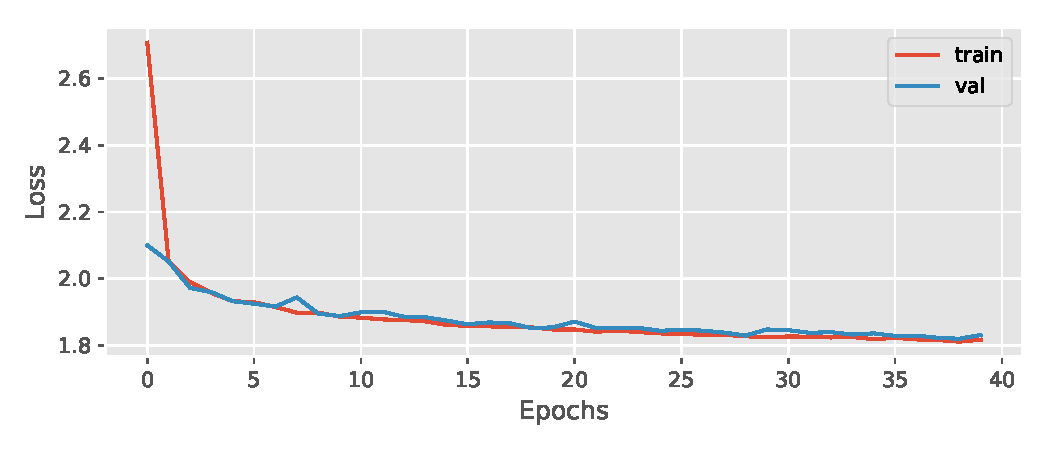
\includegraphics[width=0.7\linewidth]{assignment_3/code/figures/nf.pdf}
  \caption{The average bits per dimension during training of the normalizing flow model.}
  \label{fig:nf}
\end{figure}

\section{Conclusion}
\B{TODO: Conclusion}

\bibliographystyle{unsrtnat}
\bibliography{references}

\end{document}
